%!TEX TS-program = xelatex
%!TEX encoding = UTF-8 Unicode

\documentclass[12pt]{article}
\usepackage{geometry}                % See geometry.pdf to learn the layout options. There are lots.
\geometry{a4paper,top=2cm}
\usepackage[parfill]{parskip}    % Activate to begin paragraphs with an empty line rather than an indent
\usepackage{graphicx}
\usepackage{amsmath}
\usepackage{amssymb}
\usepackage{physics}
\usepackage{polyglossia}
\setdefaultlanguage{portuguese}

\usepackage{fontspec,xltxtra,xunicode}
\defaultfontfeatures{Mapping=tex-text}

\title{Mecânica Quântica Avançada\\Prova 01}
%\author{The Author}
\date{}

\begin{document}
\maketitle
\vspace*{-3em}

\textbf{Exercício 1:} para cada estado de dois spins-$\frac{1}{2}$ abaixo, escrito em termos dos autovetores de $S_z$, diga se o estado é emaranhado ou não (justificando sua resposta) e calcule sua matriz densidade explicitamente (\textit{i.e.} uma matriz $4\times4$).

\textbf{(a)} $\ket{\psi} = \frac{1}{\sqrt{2}}(\ket{+-}-\ket{-+})$.

\textbf{(b)} $\ket{\psi} = \ket{++}$.

\vspace*{1em}

\textbf{Exercício 2:} Considere um \emph{ensemble} estatístico de sistemas de spin-$\frac{1}{2}$.

\textbf{(a)} Considere que o ensemble é um estado puro, apontando em uma direção $\hat{n}$ (ver figura), e descrito por um ket $\alpha$. Suponha que os valores esperados $\ev{S_x}$ e $\ev{S_z}$ são conhecidos, mas apenas o \emph{sinal} de $\ev{S_y}$ é conhecido. Construa explicitamente a matriz densidade $2\times2$ que descreve o sistema. Porque é desnecessário saber a magnitude de $\ev{S_y}$?

\medskip

\begin{minipage}{0.4\textwidth}
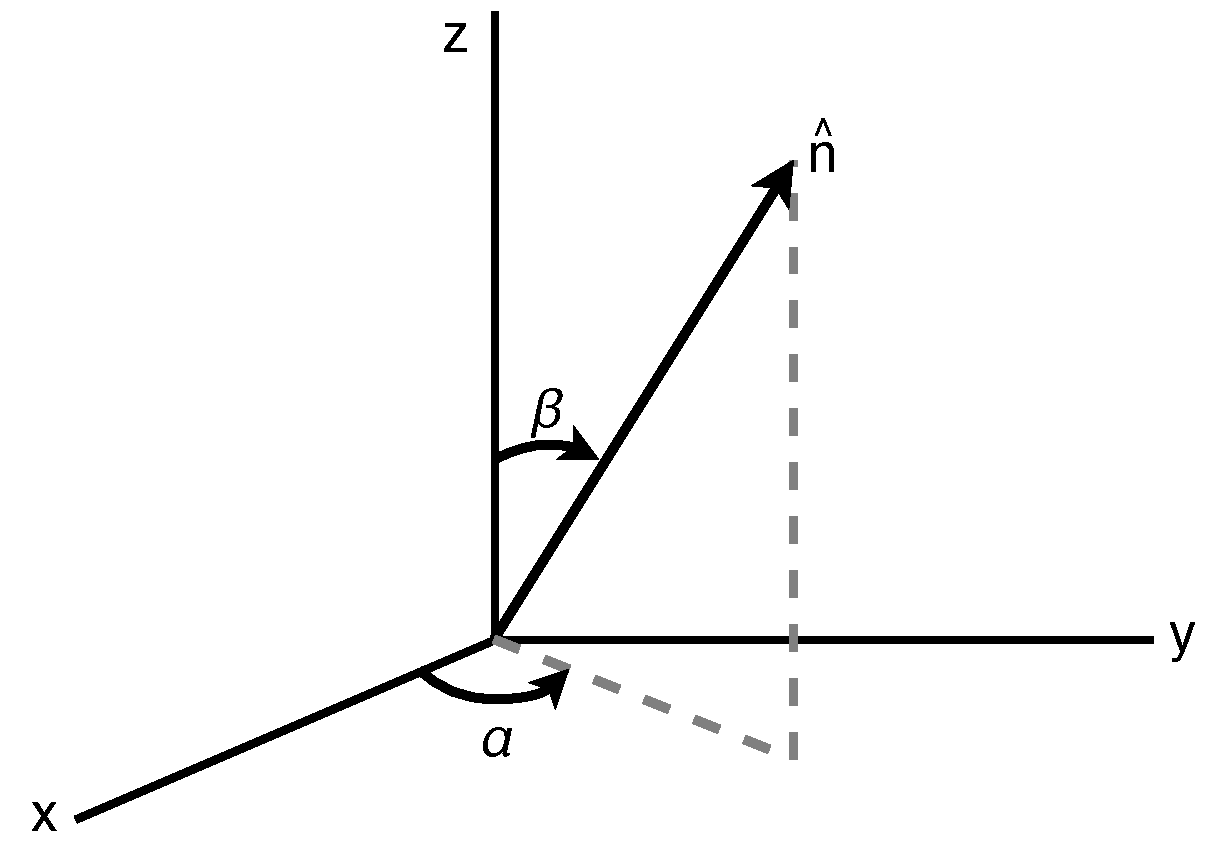
\includegraphics[width=\textwidth]{Figures/nVersor.pdf}
\end{minipage}%
\begin{minipage}{0.6\textwidth}
Estado puro apontando na direção $\hat{n}$:
\[
|\alpha\rangle=\cos \left(\frac{\beta}{2}\right)|+\rangle+e^{i \alpha} \sin \left(\frac{\beta}{2}\right)|-\rangle
\]
\end{minipage}

\medskip

\textbf{(b)} Considere agora que o ensemble é misturado, de uma maneira genérica. Suponha agora que os três valores médios
$\ev{S_x}$, $\ev{S_y}$, $\ev{S_z}$ são todos conhecidos. Construa explicitamente a matriz densidade $2\times2$ que descreve o sistema.

\vspace*{1em}

\textbf{Exercício 3:} Considere a seguinte matriz densidade de dois spins-$\frac{1}{2}$:
\[
\rho=\frac{1}{8} \mathbf{1}+\frac{1}{2}\left|\Psi_{-}\right\rangle\left\langle\Psi_{-}\right|
\]
onde \(\left|\Psi_{-}\right\rangle\) é o estado singleto (\textit{i.e.} o estado de spin total igual a zero). Suponhamos que
medimos um dos spins ao longo de um eixo \(a\) e o outro ao longo de um eixo \(b\), em que
\(\hat{a} \cdot \hat{b}=\cos \theta\). Qual é a probabilidade (como função de \(\theta\)) de encontramos \(+\hbar / 2\) para ambos
spins nestas medidas?

\textbf{Exercício 4: Interferometria de Ramsey.} Suponha que um sistema de dois níveis tem estados $\ket{+}$ e $\ket{-}$.

\textbf{(a)} Vamos considerar a chamada interação de \textit{beam splitter (BS).} Suponha que o sistema é sujeito a um Hamiltoniano $H = \epsilon \sigma_y$ por um tempo $\tau$ tal que $\epsilon \tau /\hbar = \pi/4$.
Mostre que se o sistema estava inicialmente em $\ket{+}$ ou $\ket{-}$, então ele é levado (a menos uma fase global) para os estados:
\[
\ket{+} \to \frac{\ket{+} + \ket{-}}{\sqrt{2}}
\quad,\quad
\ket{-} \to \frac{\ket{+} - \ket{-}}{\sqrt{2}}.
\]

\textbf{(b)} Agora, consideremos a chamada \textit{phase shift gate (PS)}. Suponha agora que o sistema é sujeito a um Hamiltoniano $H = \epsilon \sigma_z$ por um tempo $\tau$ tal que $\epsilon \tau /\hbar = \phi/2$. Mostre que isso leva os vetores (a menos de uma fase global) em
\[
\ket{+} \to \ket{+}\quad,\quad\ket{-} \to \exp(i\phi)\ket{-}.
\]

\textbf{(c)} Considere um sistema inicialmente preparado em $\ket{\psi_0} = \ket{+}$. Suponha agora que esse sistema evolui por um beam splitter, seguido de um phase shift, seguido de outro beam splitter, evoluindo até um estado $\ket{\psi}$. (Note que isto é possível em laboratório, usando por exemplo um sistema de spin-1/2 e um campo magnético dependente do tempo.)
\[
\ket{\psi_0} \to BS \to PS \to BS \to \ket{\psi}
\]
Calcule o estado final $\ket{\psi}$. 

\textbf{(d)} Mostre que a probabilidade $P_1$ de encontrar o sistema no estado $\ket{-}$ depois da evolução é dada por
\[
P_- = |\bra{-}\ket{\psi}|^2 = \sin^2(\phi/2).
\]
Essa é a ideia principal por trás da interferometria de Ramsey: a probabilidade oscila
dependendo da fase do phase shift.

\vfill
\par\noindent\rule{\textwidth}{0.4pt}

\textbf{Formulário}

Matrizes de Pauli:
\[
\sigma_x = \begin{pmatrix}0&1\\1&0\end{pmatrix},\,
\sigma_y = \begin{pmatrix}0&-i\\i&0\end{pmatrix},\,
\sigma_z = \begin{pmatrix}1&0\\0&-1\end{pmatrix}\quad
\begin{aligned}
\left[\,\sigma_{i}\,, \sigma_{j}\,\right]&=2 i \varepsilon_{i j k} \sigma_{k}\\
\left\{\sigma_{j}, \sigma_{k}\right\}&=2 \delta_{j k}\mathbf{I}
\end{aligned}
\]

Exponencial com matrizes de Pauli: $\exp (i \theta \vec{v} \cdot \vec{\sigma})=\cos (\theta) I+i \sin (\theta) \vec{v} \cdot \vec{\sigma}$

Evolução temporal: $\ket{\psi(t)} = \exp(\frac{-i\hat{H}t}{\hbar}) \ket{\psi(0)}$

Matriz densidade: $\hat{\rho} = \sum_\alpha p_\alpha\op{\varphi_\alpha}{\varphi_\alpha}$; lembre que $\hat{\rho}=\hat{\rho}^{\dagger}$, $\Tr\hat{\rho} = 1$.

Valor médio $\!\ev*{\hat{A}}=\Tr(\hat{\rho}\hat{A})$.

Para sistema de dois níveis:
\[\rho = 
\begin{pmatrix}
a & c\\c^*& 1-a
\end{pmatrix},\,a\text{ real},\,c\text{ complexo}
\]
\end{document}